\section{Signaling Protocol}

As we have already mentioned on our related work, \ac{WebRTC} does not implement the signaling protocol, which is used to establish connections between peers. This connection may be direct using \ac{STUN} or relayed by a \ac{TURN} server in case of direct communications are not possible.

The signaling protocol plays a fundamental role on our solution. Taking into account the choices we have based on our related work, we have decided to implement our own signaling protocol in order to use \ac{WebRTC} on our solution.

Although we have mentioned that the signaling protocol is used to establish connections between peers, on our system our media server (\ac{KMS}) is a peer that receives video streams and sends to its connected clients. 

In a general view, the signaling protocol is used to share connection and media properties between two peers. In order to ease the understanding of our signaling protocol, we have created a sequence diagram that is represented on Figure \ref{fig:signaling2}\footnote{Although two \ac{ICE} servers are shown they are, in fact, the same. Showing just one \ac{ICE} server would be difficult to draw.}.
%RP devias começar com uma introdução a explicar que tiveste de desenvolver um protocolo para coordenar a interacção dos clientes com o servidor e entre clientes (?).
%RP explicar quando é usado (começar chamada, terminar, juntar, chat(?), edição colaborativa (?), etc).
%HR done


\begin{figure}
    \centering
    \begin{subfigure}{}
    	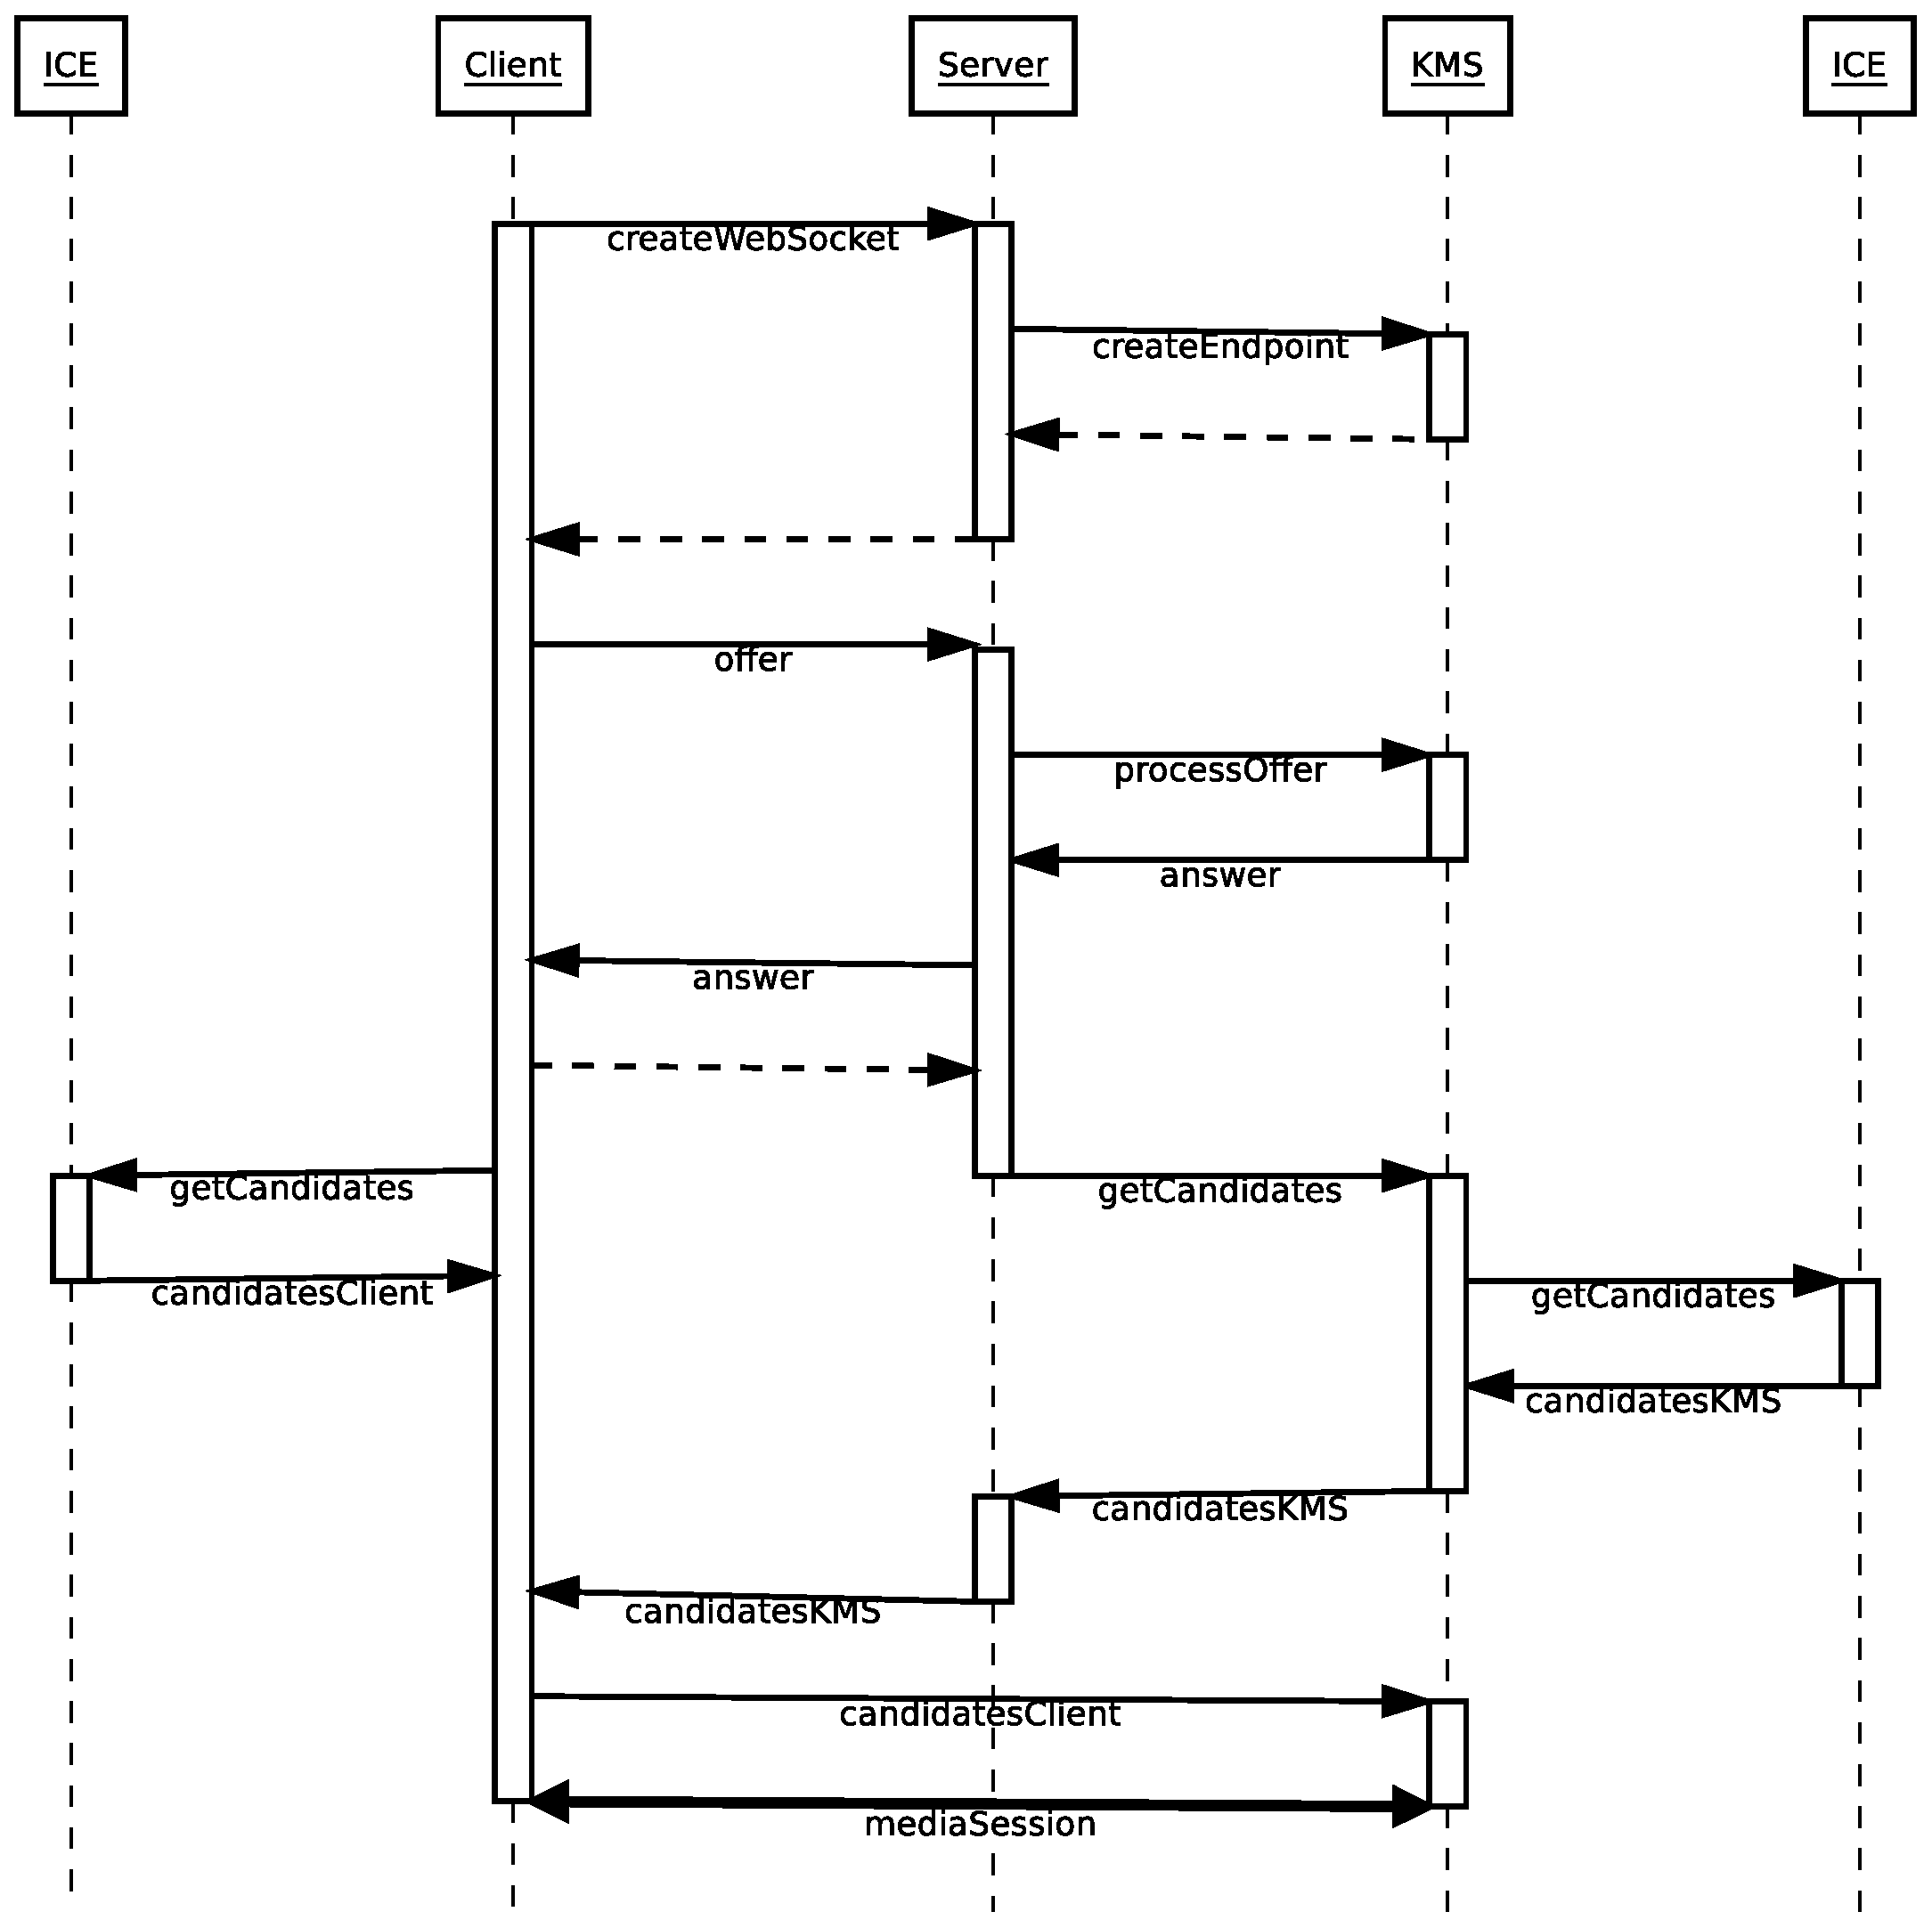
\includegraphics[width=0.9\textwidth]{figures/signaling}
    \end{subfigure}
    \caption{Signaling sequence diagram}
    \label{fig:signaling2}
\end{figure} 


%RP faz sentido haver dois ICE? Se queres colocar 2 dá-lhes nomes diferentes (nem que seja cliente e servidor ou 1 e 2).

After the web application server validates the user access, the signaling protocol allows the users to directly connect to the \ac{KMS}, which is placed in a private network, and lets the application server and users negotiate media types and encoding information to use during the conversation.
%RP o it em ``it allows'' é quem? webserver ou signaling protocol?
%HR done
We considered implementing the signaling protocol using \ac{HTTP} messages.
However, they would transport extra information such as \ac{HTTP} headers and would follow a request-response signaling mechanism which would not be the best option, as multiple ICE candidates can arrive at any time. Using a \ac{REST} \ac{API} over \ac{HTTP} for signaling and allowing other methods to be called at the same time would lead to opening multiple \ac{TCP} connections at the same time.

Instead, if we create a \emph{WebSocket} \ac{API}, we only need one \ac{TCP} connection and, at the same, provide bi-directional communications without additional headers. Moreover, using \emph{WebSocket} allows the application server to send messages asynchronously to the client without the client having to request it, which can be slightly faster than using \ac{HTTP} which is based on a request followed by a response.
%RP em vez de slighhtly faster não queres antes enfatizar que pode ser antes o servidor a iniciar a comunicação, de forma assincrona?
%HR done
Our signaling protocol consists of sending and receiving \ac{JSON} formated messages, \emph{e.g.} Listing \ref{lst:msgtype}, over WebSockets by both the application server and the client. 

\begin{minipage}{\linewidth}
\begin{lstlisting}[caption={General structure of our WebSocket messages},label={lst:msgtype},language=json]
{
	"cmd":<cmd>,
	"data":<data>
}
\end{lstlisting}
\end{minipage}

When a user enters a group conference, after the page is completely loaded, a WebSocket is created to maintain a connection with our web servers. 
But before creating the web socket, we must identify the user and check if he has permissions to participate in the conference. The user identification is done by retrieving the session id from the cookie provided by the user-agent (web browser) through the \ac{HTTP} headers.
%RP não é bem o user que fornece o cookie. é o user-agent (browser). Convém ser preciso.
%HR done
The Web application server retrieves all the information needed from the database in order to check if the user has permissions to join that conference room. It is important to save the user identification before the \emph{WebSocket} connection is created because, after the handshake is performed by the \emph{WebSocket} protocol\cite{rfc6455}, the \ac{HTTP} context is lost.
%RP socket -> websocket?

When the connection is established between the application server and the client, a \emph{PeerConnection} is created on the client and immediately after, an \ac{WebRTC} endpoint is created on the server, specifying a possible set of \ac{ICE} servers to connect.
%RP Usa Application server e não apenas server. Há muitos servers.

At this stage, the web application's user is asked if he wants to share its camera and microphone, share screen or just receive streams from the server. If the user decides to perform a screen share, \emph{adapter.js}\footnote{\url{https://github.com/Temasys/AdapterJS}(accessed March 15, 2016).} may ask to install a plug-in if the browser does not support screen sharing \footnote{\url{http://iswebrtcreadyyet.com/} (Accessed May 11, 2016)}.
%RP web app user? OU apenas client user?
%RP foot note com exemplos de browsers que aceitem screen sharing?
%HR done
If the user decides to share either from camera or screen, \emph{getUserMedia} is called with the correspondent constraints in order to obtain a local stream. We use the constraints presented on Listing \ref{lst:constraints}. 

\begin{minipage}{\linewidth}
\begin{lstlisting}[caption={Media constraints},label={lst:constraints},language=JavaScript]
var screenShareConstraints = {	
	"video": {
		"mediaSource": "window" || "screen"
	}, 
	"audio": false
};
var cameraMicrophoneConstraints = {
	"audio":true, 
	"video":true 
};
var receiveOnlyConstraints = {
	"offerToReceiveAudio":true,
	"offerToReceiveVideo":true
};
\end{lstlisting}
\end{minipage}

If the user decides to share his camera or screen, a pop-up is raised in order to ask the user to give permission to share those resources. If the resources are shared successfully, the user agent creates an offer like Listing \ref{lst:sig01}, sets a \emph{local session description} to its \emph{PeerConnection} and sends it through the WebSocket to the Application Server.
%RP usas ``user'' duas vezes, uma para te referires ao utilizador e outra ao browser (user agent).
If the resources are not shared or the user specified to receive stream only, an \ac{SDP} offer is created specifying the constraints for receiving only video and audio.
%RP offer -> SDP offer?

\begin{minipage}{\linewidth}
\begin{lstlisting}[caption={Offer created by client},label={lst:sig01},language=json]
{
	"cmd":"offer",
	"data":{
		"type":"offer",
		"sdp":<sdp>	// omitted for brevity
	}
}
\end{lstlisting}
\end{minipage}

The \emph{local session description} contains the session identifier, codecs, containers, transport protocols and ports used per media type. The \emph{local session description} is useful to conclude if the client is receiving only, which means that \ac{KMS} does not need to mix, record nor analyze streams coming from the user's \ac{WebRTC} endpoint. 

The server receives and processes the offer and sets the \emph{remote session description} to its client associated \ac{WebRTC} endpoint. Then a \emph{local session description}, like the one presented in Listing \ref{lst:sig02}, is created on the server and sent back to the client. After that, the server tries to gather \ac{ICE} candidates.
%RP listing -> Listing

\begin{minipage}{\linewidth}
\begin{lstlisting}[caption={Answer created by KMS},label={lst:sig02},language=json]
{
	"cmd":"answer",
	"data":{
		"type":"answer",
		"sdp":<sdp>	// omitted for brevity
	}
}
\end{lstlisting}
\end{minipage}

The client receives the server answer, sets the \emph{remote session description} and gets the ice candidates from the \ac{ICE} server.
%RP tens ``ice'', ``\ac{ICE}''. Acho que também já vi ``ICE''. Convém ser sempre igual!

Subsequently, after a while both the server and client receive the \ac{ICE} candidates that allow the client to connect directly to \ac{KMS} and vice-versa. The candidates are received at the client which sets them to its \emph{PeerConnection}. The same is done on the server which receives the \ac{ICE} candidates like on Listing \ref{lst:sig03} from the client and propagates them to \ac{KMS}.
%RP A figura 4.1 precisa de vir antes deste texto todo, para ser mais fácil de perceber.
%RP também tens de explicar porque razão escolheste colocar o KMS numa rede privada. Se está numa rede privada, usas NAT ou um proxy (socket) para estabelecer a ligação?
%HR uso NAT, falei disso na arquitectura, serve para o cliente não aceder directamente ao servidor de streaming e realizar o seu proprio protocolo de sinalizacao (uso indevido por parte de atacantes)

\begin{minipage}{\linewidth}
\begin{lstlisting}[caption={ICE candidates sent by KMS and client},label={lst:sig03},language=json]
{
	"cmd":"iceCandidate",
	"data":{
		"sdpMLineIndex":0,
		"candidate":"candidate:15 1 TCP 843056127 146.193.224.20 48828 typ srflx raddr 192.168.1.105 rport 48828 tcptype passive",
		"sdpMid":"audio"
	},
}
\end{lstlisting}
\end{minipage}

An \ac{ICE} candidate contains an \ac{IP}, port, used transport protocol and an attribute named \emph{sdpMLineIndex} that is used for mapping to the \emph{remote session description} media type.
In addition, both intervenients test the connectivity of each \ac{ICE} candidate. When a connection is established, the user and server start to interchange stream data but other \ac{ICE} candidates may arrive with better connections. When that happens, the connection changes seamlessly. 

Having the media session established, the server starts to record any received stream and the client creates an \ac{URL} correspondent to the stream location.


%RP não falas nada sobre chats, etc! Não há signalling para isso?
%HR não, só video e audio, chat é websockets